\chapter{Symmetric and PSD Matrices}
\label{ch:symmetric-psd}

\section{Quadratic Forms}

The expression
\[
  x^TAx
\]
is a \emph{quadratic form}. It takes a vector as input and returns a scalar.
For example, if
\[
  A=\begin{bmatrix}2&1\\1&2\end{bmatrix},
  \qquad
  x=\begin{bmatrix}x_1\\x_2\end{bmatrix},
\]
then
\[
  x^TAx=2x_1^2+2x_1x_2+2x_2^2.
\]

Quadratic forms are where matrices meet geometry. They describe squared
lengths, energies, variances, and second-order approximations.

\begin{figure}[htbp]
  \centering
  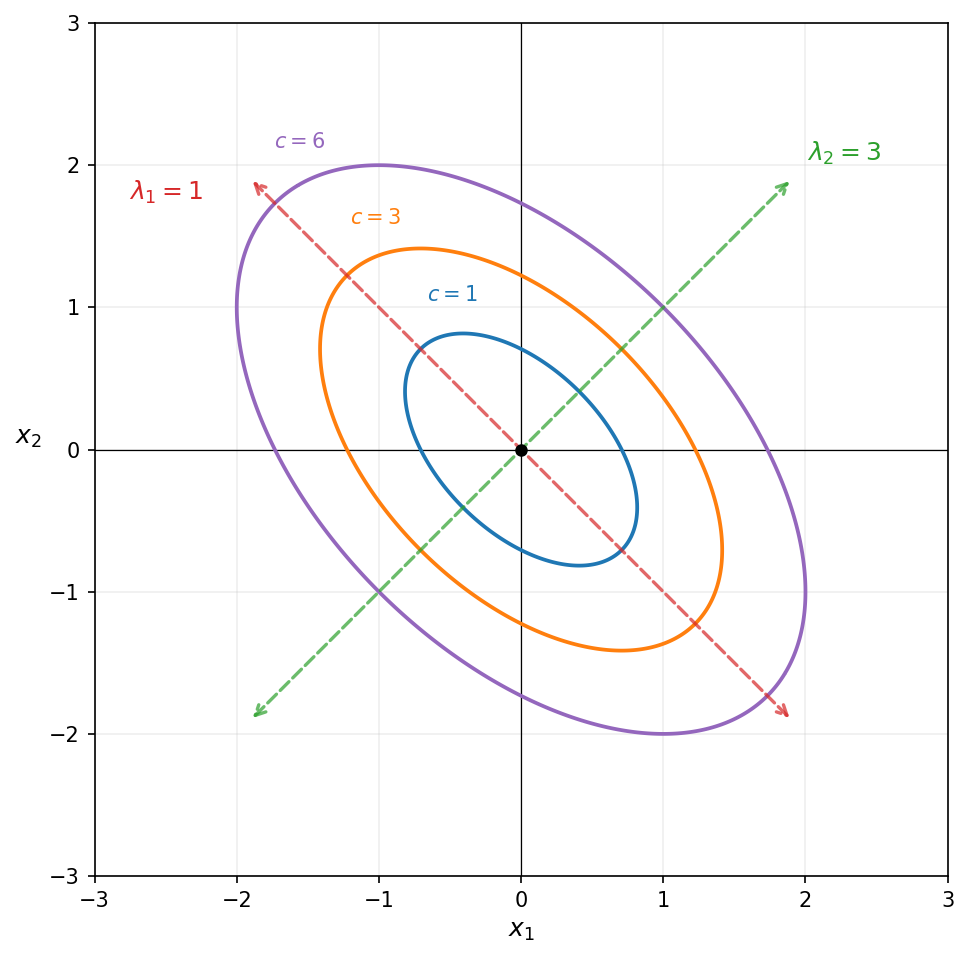
\includegraphics[width=0.68\textwidth]{book/assets/figures/core/fig08_psd_quadratic.png}
  \caption{Level curves $x^TAx=c$ for a symmetric positive definite matrix.
  The ellipse axes point in eigenvector directions. Larger eigenvalues produce
  shorter axes for the same value of $c$.}
\end{figure}

\section{Symmetric Matrices}

\begin{definition}[Symmetric matrix]
A real square matrix $A$ is \emph{symmetric} if
\[
  A^T=A.
\]
\end{definition}

Symmetric matrices are special because the input and output geometry match.
They are the matrices for which the spectral theorem will give an orthonormal
eigenbasis.

\begin{example}
The matrix
\[
  \begin{bmatrix}2&1\\1&2\end{bmatrix}
\]
is symmetric. The matrix
\[
  \begin{bmatrix}2&3\\1&2\end{bmatrix}
\]
is not.
\end{example}

\section{Positive Semidefinite Matrices}

\begin{definition}[Positive semidefinite]
A symmetric matrix $A\in\R^{n\times n}$ is \emph{positive semidefinite}, or
PSD, if
\[
  x^TAx\geq 0
  \qquad\text{for every }x\in\R^n.
\]
It is \emph{positive definite}, or PD, if
\[
  x^TAx>0
  \qquad\text{for every nonzero }x\in\R^n.
\]
\end{definition}

\begin{example}
The matrix
\[
  A=\begin{bmatrix}2&0\\0&-1\end{bmatrix}
\]
is not PSD, because with $x=(0,1)^T$,
\[
  x^TAx=-1.
\]
\end{example}

\begin{proposition}
For every real matrix $B$, the matrix $B^TB$ is symmetric and PSD.
\end{proposition}

\begin{proof}
Symmetry:
\[
  (B^TB)^T=B^T(B^T)^T=B^TB.
\]
For any $x$,
\[
  x^TB^TBx=(Bx)^T(Bx)=\norm{Bx}^2\geq 0.
\]
\end{proof}

This proposition explains why $A^TA$ appeared in the normal equations. It is
not just a convenient square matrix; it is symmetric PSD.

\section{Kernel And Positive Definiteness}

\begin{proposition}
For every real matrix $B$,
\[
  \Ker(B^TB)=\Ker(B).
\]
\end{proposition}

\begin{proof}
If $Bx=0$, then $B^TBx=0$. Conversely, if $B^TBx=0$, multiply on the left by
$x^T$:
\[
  0=x^TB^TBx=\norm{Bx}^2.
\]
Thus $Bx=0$.
\end{proof}

\begin{corollary}
If $B$ has linearly independent columns, then $B^TB$ is positive definite.
\end{corollary}

\begin{proof}
If $x\neq 0$ and the columns of $B$ are independent, then $Bx\neq 0$. Hence
\[
  x^TB^TBx=\norm{Bx}^2>0.
\]
\end{proof}

\section{Gram Matrices}

\begin{definition}[Gram matrix]
Given vectors $v_1,\ldots,v_n$ in an inner product space, their \emph{Gram
matrix} is
\[
  G_{ij}=\inner{v_i}{v_j}.
\]
\end{definition}

If $B$ has columns $v_1,\ldots,v_n$ in $\R^m$, then
\[
  G=B^TB.
\]
Therefore every Gram matrix is symmetric PSD.

\begin{aimlbox}
Gram matrices appear whenever data are represented through pairwise inner
products or similarities. The linear algebra point is simple and important:
any matrix of exact dot products must be PSD.
\end{aimlbox}

\section{Covariance Matrices}

Let $X\in\R^{N\times d}$ be a centered data matrix: rows are samples, columns
are features, and each column has mean zero. The sample covariance matrix is
often written as
\[
  C=\frac{1}{N-1}X^TX.
\]
By the proposition above, $C$ is symmetric PSD.

For any direction $w\in\R^d$,
\[
  w^TCw=\frac{1}{N-1}\norm{Xw}^2\geq 0.
\]
This number is the variance of the data after projecting each sample onto the
direction $w$.

\section{Trace}

\begin{definition}[Trace]
The trace of a square matrix is the sum of its diagonal entries:
\[
  \Trace(A)=a_{11}+a_{22}+\cdots+a_{nn}.
\]
\end{definition}

For a covariance matrix, the diagonal entries are the variances of the
individual features. Therefore
\[
  \Trace(C)
\]
is the total feature variance.

\begin{proposition}[Cyclic trace rule]
If the products are defined and square, then
\[
  \Trace(AB)=\Trace(BA).
\]
\end{proposition}

\begin{proof}
If $A\in\R^{m\times n}$ and $B\in\R^{n\times m}$, then
\[
  \Trace(AB)
  =
  \sum_{i=1}^m (AB)_{ii}
  =
  \sum_{i=1}^m\sum_{j=1}^n A_{ij}B_{ji}.
\]
Changing the order of summation gives
\[
  \sum_{j=1}^n\sum_{i=1}^m B_{ji}A_{ij}
  =
  \Trace(BA).
\]
\end{proof}

\begin{corollary}
Similar matrices have the same trace:
\[
  \Trace(P^{-1}AP)=\Trace(A).
\]
\end{corollary}

\begin{proof}
\[
  \Trace(P^{-1}AP)=\Trace(APP^{-1})=\Trace(A).
\]
\end{proof}

\section{Python Thread}

\begin{lstlisting}
import numpy as np

rng = np.random.default_rng(0)
B = rng.standard_normal((5, 3))
A = B.T @ B

print("symmetric:", np.allclose(A, A.T))
print("eigenvalues:", np.linalg.eigvalsh(A))

for _ in range(5):
    x = rng.standard_normal(3)
    print(x @ A @ x)

# Centered data and covariance
X = rng.standard_normal((100, 4))
X = X - X.mean(axis=0)
C = X.T @ X / (X.shape[0] - 1)

print("covariance PSD eigenvalues:", np.linalg.eigvalsh(C))
print("total variance:", np.trace(C))
print("sum of feature variances:", np.sum(np.var(X, axis=0, ddof=1)))
\end{lstlisting}

\begin{labbox}
The PCA part of Lab 10 uses covariance matrices. The key facts needed there
are already here: covariance matrices are PSD, their quadratic forms measure
variance in directions, and their trace measures total variance.
\end{labbox}

\section*{Chapter Summary}
\addcontentsline{toc}{section}{Chapter Summary}

\begin{itemize}
  \item Quadratic forms $x^TAx$ turn matrices into scalar measurements.
  \item A symmetric matrix is PSD if $x^TAx\geq 0$ for every $x$.
  \item $B^TB$ is always symmetric PSD.
  \item Gram and covariance matrices are PSD.
  \item The trace of a covariance matrix is total variance.
\end{itemize}

\section*{Exercises}
\addcontentsline{toc}{section}{Exercises}
\subsection*{A. Theory}
\begin{exercise}\exerciseid{12.A1} Prove that if $Av=\lambda v$ and $v\neq 0$, then $A^kv=\lambda^kv$ for every integer $k\geq 0$. \end{exercise}
\subsection*{B. By Hand}
\begin{exercise}\exerciseid{12.B1} Find the eigenvalues and eigenvectors of $\mat{2&0\\0&3}$. \end{exercise}
\subsection*{C. Python / NumPy}
\begin{exercise}\exerciseid{12.C1} Use \texttt{np.linalg.eig} on a diagonal matrix and on a non-diagonal matrix with known eigenvectors. \end{exercise}
\subsection*{D. Challenge}
\begin{exercise}\exerciseid{12.D1} Give a $2\times 2$ matrix with only one eigenvector direction. \end{exercise}

